\chapter{Combining NSB with the Hand Position Approach}
\label{chap:handpos_NSB}

This chapter presents an extended \acrfull{nsb} algorithm for the formation control of fleets of underactuated autonomous underwater vehicles. 
The \gls{nsb} controller is developed to work directly with second-order integrator systems, handling the double integrator dynamics in task space. 
The method is applied to the formation path-following problem of a fleet of underactuated autonomous underwater vehicles. 
The nonlinear six-degrees-of-freedom models of the vehicles are transformed into second-order integrator systems using the 3D hand position output linearizing approach presented in Chapter~\ref{chap:handpos_definition}. 
The behavioral controller implements a hierarchy of path-following, formation-keeping, and collision-avoidance tasks.
The closed-loop system is proven \acrlongpl{ugas}, and the proposed method is validated through numerical simulations.
The contents of this chapter are based on \cite{lie_formation_2023}.

\section{Introduction}

The \gls{nsb} algorithm, as presented in the existing literature, is developed for kinematic single-integrator systems \cite{arrichiello_formation_2006,matous_singularity_2023,eek_formation_2021}. In this work, we extend the \gls{nsb} method to vehicles with double integrator dynamics and propose an algorithm that uses the \acrlong{soclik} equation to control the task variables through desired acceleration. The procedure is inspired by robotic manipulators, where second-order methods are more common,  due to the inherent second-order dynamics of mechanical systems \cite{siciliano_differential_2009, chiaverini_kinematically_2008}. Although existing \gls{nsb} methods are developed for first-order systems, \gls{auv} dynamics are inherently second-order. Therefore, any first-order solution is necessarily perturbed by the dynamics of the maneuvering controller. In contrast, our formulation handles the second-order dynamics directly in the task space as interpretable spring-damper systems.

We apply the proposed \gls{nsb} method to a fleet of \glspl{auv}. \Glspl{auv} are underactuated systems with inherently nonlinear dynamics. What enables us to still use the proposed \gls{nsb} method, developed for vehicles with linear double integrator dynamics, is the use of the hand position input-output linearization method presented in Chapter~\ref{chap:handpos_definition}. Subsequently, through the design of specific path-following, formation-keeping, and collision-avoidance tasks, the fleet is controlled to follow a preplanned path in formation while avoiding collisions both within the fleet and with external obstacles. The stability of the system is proved, and its effectiveness is verified in simulation. Because our reformulated NSB method works directly with the second-order system given by the hand position controller, there is no need to transform desired velocities or accelerations into surge and orientation references, as has been done in previous works. This reduces one level of complexity in the controller design.

This chapter is organized as follows. Section \ref{sec:NSB} presents the extended \gls{nsb} algorithm which is applicable for general double-integrator systems. Section \ref{sec:case_study} presents a case study of this \gls{nsb} algorithm applied to a fleet of \glspl{auv}. Section \ref{sec:conclusion} presents some concluding remarks.

\section{The NSB Algorithm for Double Integrators}\label{sec:NSB}
The \gls{nsb} method enables the creation of multiple tasks in a hierarchical manner, ensuring that low-priority tasks do not interfere with high-priority ones. In this section, we extend this method to second-order systems with double integrator dynamics.
This modified \gls{nsb} algorithm provides the acceleration input $\bm{\mu}$ to the following system
\begin{subequations}
    \begin{align}
        \dot{\mathbf{p}} &= \ivel, \\
        \dot{\ivel} &= \bm{\mu}.
    \end{align}
\end{subequations}

For each task, we design a task variable $\bm{\sigma}_i \in \mathbb{R}^m_i$ as a function of $\mathbf{p}$
\begin{equation}
    \bm{\sigma}_i = \mathbf{f}_i(\mathbf{p}).
\end{equation}
The first and second time-derivatives of $\bm{\sigma}_i$ are
\begin{subequations}\label{eq:task_derivatives}
    \begin{align}
        \dot{\bm{\sigma}}_i &= \mathbf{J}_i(\mathbf{p})\ivel,\\
        \ddot{\bm{\sigma}}_i &= \mathbf{J}_i(\mathbf{p})\dot{\ivel} + \dot{\mathbf{J}}_i \ivel,\label{eq:task_second_derivative}
    \end{align}
\end{subequations}
where $\mathbf{J}_i = \partial \mathbf{f}_i/\partial \mathbf{p}$ is the task Jacobian. We denote the desired value of the task variable by $\bm{\sigma}_{d, i}$.

In Section~\ref{sec:background_NSB}, we introduced the \acrfull{clik} equation as a method for finding the desired velocity associtated with a given task.
Recalling \eqref{eq:background_CLIK}, the desired velocity of task $i$, $\ivel_i$, is given by
\begin{equation}
    \ivel_i = \mathbf{J}_i^\dagger\bigl(\dot{\bm{\sigma}}_{d, i} - \bm{\Lambda}_i \Tilde{\bm{\sigma}}_i\bigr),
\end{equation}
where $\bm{\Lambda}_i$ is a positive definite gain matrix, $\Tilde{\bm{\sigma}}_i = \bm{\sigma}_i - \bm{\sigma}_{d,i}$ is the task error, and $\mathbf{J}_i^\dagger$ is the pseudo-inverse of the task Jacobian. 
To achieve second-order differential control, we instead propose the \gls{soclik} equation inspired by robotic manipulators \cite{siciliano_closed-loop_1990}
\begin{equation}
    \dot{\ivel}_i = \mathbf{J}_i^\dagger \bigl(\ddot{\bm{\sigma}}_{d,i} - \mathbf{\Lambda}_{p,i}\Tilde{\bm{\sigma}}_i - \mathbf{\Lambda}_{d,i} \dot{\Tilde{\bm{\sigma}}}_i - \dot{\mathbf{J}}_i \ivel\bigr), \label{eq:general_acceleration}
\end{equation}
where $\mathbf{\Lambda}_{p,i}$ and $\mathbf{\Lambda}_{d,i}$ are positive definite gain matrices.

In first-order systems, there exists a subspace of velocities that do not conflict with a given task.
Similarly, in second-order systems, there exists a subspace of non-conflicting accelerations.
Let $\dot{\ivel}_i$ be the \gls{soclik} solution to task $i$, and let $\dot{\ivel}_{\rm add}$ be some additional desired acceleration.
Then, the following control input
\begin{equation}
    \dot{\ivel} = \dot{\ivel}_i +\mathbf{N}_i \dot{\ivel}_{\rm add},
    \label{eq:NSB_two_tasks}
\end{equation}
where $\mathbf{N}_i$ is the null space projector of the task, guarantees the desired behavior of the task.

Similarly to first-order \gls{nsb} methods, we can combine the tasks by projecting the inputs from the lower-priority tasks onto the null space of the higher-priority tasks.
The desired acceleration is then given by
\begin{equation}
    \bm{\mu} = \dot{\ivel}_1 + \sum_{i=2}^N \bar{\mathbf{N}}_{i-1}\dot{\ivel}_i,
    \label{eq:NSB_double}
\end{equation}
where $\bar{\mathbf{N}}_i$ is the null space projector of the augmented Jacobian \eqref{eq:background_NSB_augmented}.
With this choice of acceleration, the highest priority task is always fulfilled, whereas the lower priority tasks are fulfilled as well as possible in the subspace that does not conflict with higher priority tasks.

\subsection{Stability Analysis}
In this section, we investigate the stability of an \gls{nsb} algorithm consisting of two tasks.
The proof is based on \cite{antonelli_stability_2008}, but extended to a double integrator system.
The proof utilizes the concepts of independence and orthogonality defined in Section~\ref{sec:background_NSB_independence}.

\begin{lemma}\label{theorem:one}
    Consider two independent and orthogonal tasks labeled 1 and 2.
    Let
    $
        \Tilde{\mathbf{X}}\T = \left[\Tilde{\bm{\sigma}}_1\T, \Tilde{\bm{\sigma}}_2\T, \dot{\Tilde{\bm{\sigma}}}_1\T, \dot{\Tilde{\bm{\sigma}}}_2\T \right]
    $
    be the stacked error vector.

    The control input defined in \eqref{eq:NSB_double} ensures that $\Tilde{\mathbf{X}} = \mathbf{0}$ is a \acrfullpl{ges} equilibrium point.
\end{lemma}

\begin{proof}
    First, let us find the closed-loop expressions for $\ddot{\Tilde{\bm{\sigma}}}_1$ and $\ddot{\Tilde{\bm{\sigma}}}_2$.
    From \eqref{eq:task_second_derivative} and \eqref{eq:NSB_double}, we get
    \begin{subequations}\label{eq:proof_second_derivatives}
        \begin{align}
            \ddot{\Tilde{\bm{\sigma}}}_1 &= \mathbf{J}_1\dot{\ivel}_1 + \mathbf{J}_1\mathbf{N}_1\dot{\ivel}_2 + \dot{\mathbf{J}}_1\ivel - \ddot{\bm{\sigma}}_{d, 1}, \\
            \ddot{\Tilde{\bm{\sigma}}}_2 &= \mathbf{J}_2\dot{\ivel}_1 + \mathbf{J}_2\mathbf{N}_1\dot{\ivel}_2 + \dot{\mathbf{J}}_2\ivel - \ddot{\bm{\sigma}}_{d, 2}, 
        \end{align}
    \end{subequations}
    Note that thanks to the independence and orthogonality assumptions, it follows that $\mathbf{J}_2 \mathbf{N}_1 \mathbf{J}_2^{\dagger} = \mathbf{I}$.
    Consequently, substituting \eqref{eq:general_acceleration} into \eqref{eq:proof_second_derivatives} and using \eqref{eq:task_derivatives}, the time-derivative of $\Tilde{\mathbf{X}}$ is given by
    \begin{align}
        \dot{\Tilde{\mathbf{X}}} &= \mathbf{M}\Tilde{\mathbf{X}}, &
        \mathbf{M} &= 
        \begin{bmatrix}
            \mathbf{O} & \mathbf{O} & \mathbf{I} & \mathbf{O} \\
            \mathbf{O} & \mathbf{O} & \mathbf{O} & \mathbf{I} \\
            -\mathbf{\Lambda}_{p,1} & \mathbf{O} & -\mathbf{\Lambda}_{d,1} & \mathbf{O} \\
            \mathbf{O} & -\mathbf{\Lambda}_{p,2} & \mathbf{O} & -\mathbf{\Lambda}_{d,2}
        \end{bmatrix}.
    \end{align}
    Since the gain matrices are positive definite by design, the matrix $\mathbf{M}$ is Hurwitz, and the closed-loop system is \glspl{ges}.
\end{proof}

\section{Case Study: Formation Path Following of AUVs}\label{sec:case_study}
The following sections present a case study of the proposed second-order \gls{nsb} algorithm applied to a fleet of underactuated \glspl{auv} equipped with the hand-position-based controller defined in Chapter~\ref{chap:handpos_definition}. The control objective of the fleet is to follow a predefined path while keeping formation and avoiding obstacles.

The vehicle model under the hand position controller is presented in Section \ref{sec:vehicle_model} and the formation path following problem is formulated in Section~\ref{sec:formation_path_following}. The NSB tasks are detailed in Section \ref{sec:NSB_case_study}, Section \ref{sec:obstacle_avoidance} details the obstacle avoidance method, Section \ref{sec:closed_loop} analyzes the stability properites, and Section \ref{sec:simulation} presents a simulation study.

\subsection{AUV Model}\label{sec:vehicle_model}
We consider a 6\gls{dof} model of an \gls{auv} exposed to an unknown constant irrotational ocean current, and apply the 3D hand position transform from Chapter~\ref{chap:handpos_definition}.
Recalling \eqref{eq:handpos_def_hand_position_dynamics}, the transformed dynamics of the \gls{auv} are
\begin{subequations}\label{eq:linearized_system}
    \begin{align}
        \dot{\mathbf{x}}_1 &= \mathbf{x}_2 + \ocean,\\
        \dot{\mathbf{x}}_2 &= \bm{\mu},\\
        \dot{\mathbf{R}} &=  \mathbf{R} \mathbf{S}(\bm{\omega}),\\
        \dot{\bs{\omega}} &= \Bar{\mat{L}} \times \left(\mat{R}\T\bs{\mu} + \mathcal{D}_{\bvel}(\vel) + \mathcal{C}_{\bvel}(\vel) - \bs{\omega} \times \mat{R}\T \mat{x}_2\right) \label{eq:internal_dynamics} \\
            & \quad - \left(\Bar{\mat{L}}\mat{L}\T\right) \left(\mathcal{D}_{\bs{\omega}}(\vel) + \mat{M}_{22}^{\prime}\left(Wz_{gb} \mat{e}_3 \times \mat{R}\T \mat{e}_3\right)\right). \nonumber
    \end{align}
\end{subequations}

%%%%%%%%%%%%%%%%%%%%%%%%%%%%%%%%%%%%%%%%%%%%%%%%%%%%%%%%%%%%%%%%%%%%%%%%%%%%%%%%
\subsection{Formation Path Following}\label{sec:formation_path_following}
The formation path-following problem considered in this chapter is analogous to the one defined in Section~\ref{sec:background_formation_path_following}.
We consider a fleet of $n$ \glspl{auv} and define the stacked position and velocity vectors $\mathbf{p} = [\mathbf{x}_{1,1}\T, \, \ldots,\, \mathbf{x}_{1,n}\T]\T$ and $\mathbf{v} = [\mathbf{x}_{2,1}\T, \, \ldots,\, \mathbf{x}_{2,n}\T]\T$, respectively. We also define the stacked ocean current vector $\stackedocean = \mathbf{1}_{n} \otimes \ocean$. In the following sections, we denote the hand position of a single \gls{auv} by $\mathbf{p}_i = \mathbf{x}_{1,i}$ and its velocity relative to the ocean current by $\mathbf{v}_i = \mathbf{x}_{2,i}$.

The desired path is parametrized by a smooth function $\mathbf{p}_p : \mathbb{R} \mapsto \mathbb{R}^3$ that is assumed to be $\mathcal{C}^\infty$ and regular.
For every point $\mathbf{p}_p(s)$, there exists a path-tangential coordinate-frame with a corresponding rotation matrix $\mathbf{R}_p$ (see Section~\ref{sec:background_paths}). 
The path-following error $\mathbf{p}_b^p$ is defined in terms of the barycenter of the fleet in the path-tangential coordinate frame
\begin{equation}
    \mathbf{p}_b^p = \mathbf{R}_p\T\left(\mathbf{p}_b - \mathbf{p}_p(s)\right), \quad \mathbf{p}_b = \frac{1}{n}\sum_{i=1}^n \mathbf{p}_i.
\end{equation}
The goal of path following is to control the vehicles so that $\mat{p}_b^p \rightarrow \mat{0}_3$.

The vehicles should converge to a dynamic formation that rotates with the desired path (see Section~\ref{sec:background_formation_keeping} for details).
Let $\mat{p}_{f,1}^f, \ldots, \mat{p}_{f,n}^f$ be the position vectors that represent the desired formation.
The objective is to control the vehicles so that
\begin{align}
    \mat{p}_i - \mat{p}_b &\rightarrow \mat{R}_p \mat{p}_{f,i}^f + \mat{p}_b, &
    i &\in \left\{1, \ldots, n \right\}.
\end{align}

\subsection{NSB Controller}\label{sec:NSB_case_study}

We let the control system consist of three tasks in decreasing order of priority: inter-vehicle collision avoidance, formation keeping, and path following. The following sections will detail the chosen task variables and \gls{soclik} solution for each task.

\subsubsection{Inter-vehicle collision avoidance}

The highest priority task is inter-vehicle \acrfull{colav}. The task variable is given by a stacked vector $\bm{\sigma}_1 = [\sigma_{1,1}\T, \ldots, \sigma_{1,l}\T]\T$ of relative distances between vehicles closer than the activation distance $d_{COLAV}$:
\begin{equation}
\begin{split}
    \sigma_{1,k} = \|\mathbf{p}_i - \mathbf{p}_j\|, \quad &\forall i,j \in {1, \ldots, n}: j > i,\\
    &\|\mathbf{p}_i - \mathbf{p}_j\| < d_{COLAV}.
    \end{split}
\end{equation}
The task size varies depending on the number of vehicles that are within the activation distance, and it is empty under nominal conditions. The desired values of the task are given by
\begin{equation}
    \bm{\sigma}_{d,1} = d_{COLAV} \mathbf{1}_l.
\end{equation}
We note that $\ddot{\bm{\sigma}}_{d,1} = \dot{\bm{\sigma}}_{d,1}= \mat{0}$.

The task Jacobian is given by the stacked partial derivatives for each active collision
\begin{subequations}
\begin{align}
    \mathbf{J}_1 &= \left[\left(\frac{\partial \sigma_{1,1}}{\partial \mathbf{p}}\right)\T, \ldots, \left(\frac{\partial \sigma_{1,l}}{\partial \mathbf{p}}\right)\T\right]\T,\\
    \frac{\partial \sigma_{1,k}}{\partial \mathbf{p}_i} &=\frac{\left(\mathbf{p}_i-\mathbf{p}_j\right) \T}{\|\mathbf{p}_i - \mathbf{p}_j\|}, \qquad
    \frac{\partial \sigma_{1,k}}{\partial \mathbf{p}_j} = -\frac{\left(\mathbf{p}_i-\mathbf{p}_j\right) \T}{\|\mathbf{p}_i - \mathbf{p}_j\|}.
\end{align}
\end{subequations}
The derivative of the task Jacobian is similarly given by a stack of time-differentiated partial derivatives
\begin{subequations}
\begin{align}
    \dot{\mathbf{J}}_1 &= \left[{\left(\frac{{\rm d}}{{\rm d}t}\frac{\partial \sigma_{1,1}}{\partial \mathbf{p}}\right)}\T, \ldots, {\left(\frac{{\rm d}}{{\rm d}t}\frac{\partial \sigma_{1,l}}{\partial \mathbf{p}}\right)}\T\right]\T,\\
    {\frac{{\rm d}}{{\rm d}t}\frac{\partial \sigma_{1,k}}{\partial \mathbf{p}_i}} &= \bigg(\frac{\mathbf{I}_3}{\|\mathbf{p}_i - \mathbf{p}_j\|} - \frac{\bigl(\mathbf{p}_i-\mathbf{p}_j\bigr)\bigl(\mathbf{p}_i-\mathbf{p}_j\bigr)\T}{\|\mathbf{p}_i - \mathbf{p}_j\|^3}\bigg)\bigl(\mathbf{v}_i-\mathbf{v}_j\bigr),
\end{align}
\end{subequations}

The resulting \gls{soclik} equation for the task is
\begin{equation}
    \dot{\mathbf{v}}_1 = -\mathbf{J}_1^\dagger \bigl( \mathbf{\Lambda}_{p,1}\Tilde{\bm{\sigma}}_1 + \mathbf{\Lambda}_{d,1} \dot{\bm{\sigma}}_1 + \dot{\mathbf{J}}_1 (\mathbf{v}+\stackedocean)\bigr),
\end{equation}
with $\dot{\bm{\sigma}}_{1\,} \!\!= \mathbf{J}_1 (\mathbf{v}\! + \!\stackedocean)$. %We note that because of the symmetry of the task and the structure of the task Jacobian, the constant ocean currents will cancel out in $\dot{\mathbf{v}}_1$ under the assumption that it is equal for all vehicles.
Note that due to the structure of the task Jacobian, it follows that $\mathbf{J}_1 \stackedocean \!\!= \dot{\mathbf{J}}_1 \stackedocean \!\!= \mathbf{0}$. Consequently, $\dot{\mathbf{v}}_1$ is independent of the ocean current velocity.

\subsubsection{Formation-keeping task}
The formation-keeping task moves the vehicles into a predefined formation in the formation-centered frame. The task variable is given by
\begin{equation}
    \bm{\sigma}_2 = \left[ \bm{\sigma}_{2,1}\T, ..., \bm{\sigma}_{2,n-1}\T\right]\T, \quad \bm{\sigma}_{2,i}  = \mathbf{p}_i - \mathbf{p}_b.
\end{equation}
The desired values are
\begin{equation}
    \bm{\sigma}_{d,2} = [\bigl(\mathbf{R}_p \mathbf{p}_{f,1}^f\bigr)\T, ..., \bigl(\mathbf{R}_p \mathbf{p}_{f,n-1}^f\bigr) \T] \T.
\end{equation}
The Jacobian is given by 
\begin{equation}
    \mathbf{J}_2 = \left(\begin{bmatrix}
        \mathbf{I}_{n-1} & \mathbf{0}_{n-1}
    \end{bmatrix} - \frac{\mathbf{1}_{(n-1) \times n}}{N}\right)\otimes \mathbf{I}_3.
\end{equation}
Because $\dot{\mathbf{J}}_2 = \mathbf{0}$, the \gls{soclik} equation reduces to
\begin{equation}\label{eq:formation_keeping_controller}
    \dot{\mathbf{v}}_2 = \mathbf{J}_2^\dagger \bigl(\ddot{\bm{\sigma}}_{d,2} - \mathbf{\Lambda}_{p,2}\Tilde{\bm{\sigma}}_2 - \mathbf{\Lambda}_{d,2} \dot{\Tilde{\bm{\sigma}}}_2\bigr).
\end{equation}
%where
%\begin{align}
 %   \dot{\bm{\sigma}}_{d,2} &= [\bigl(\dot{\mathbf{R}}_p \mathbf{p}_{f,1}^f\bigr)\T, ..., \bigl(\dot{\mathbf{R}}_p \mathbf{p}_{f,n-1}^f\bigr) \T] \T.
%\end{align}
%because the path-formation variables $\mathbf{p}_{f,i}^p$ are constant.

The nominal task acceleration \eqref{eq:formation_keeping_controller} may saturate the actuators if the formation error is large. The \gls{nsb} controller may also lead to a loss of controllability if the formation-keeping velocities exactly cancel out the path-following velocities. Therefore, similarly to Chapter~\ref{chap:NSB_R}, we introduce saturated task acceleration
\begin{equation}\label{eq:saturated_formation_keeping}
\dot{\mathbf{v}}_2 = \mathbf{J}_2^\dagger \bigl(\ddot{\bm{\sigma}}_{d,2} - v_{2_{\max}}\mathrm{sat}\bigl(\mathbf{\Lambda}_{p,2}\Tilde{\bm{\sigma}}_2\bigr) - \mathbf{\Lambda}_{d,2} \dot{\Tilde{\bm{\sigma}}}_2\bigr),
\end{equation}
where $v_{2_{\max}}$ is a positive constant and $\mathrm{sat}$ is a saturation function given by
\begin{equation}
    \mathrm{sat}\bigl(\mathbf{x}\bigr) = \mathbf{x}\frac{\tanh{\|\mathbf{x}\|}}{\|\mathbf{x}\|}.
\end{equation}
With the saturated task acceleration, we further require that the product of the gain matrices $\mathbf{\Lambda}_{p,2} \mathbf{\Lambda}_{d,2}$ is symmetric positive definite.
Similarly to the inter-vehicle collision avoidance task, this task is independent of the ocean current.% because it concerns the relative movement of the vehicles in relation to each other.

\subsubsection{Path-following task}
The path following task concerns moving the barycenter along the predefined path. Moreover, we want the formation to move at a constant, desired path-following speed $U_{LOS}$. We apply the same acceleration to all vehicles to ensure that the barycenter moves without changing the relative formation.

We apply the coupled \acrfull{los} guidance algorithm defined in Section~\ref{sec:background_LOS}, and modify it to work with double-integrator systems. We denote the components of the path following error $\mathbf{p}_b^p$ as $x_b^p$, $y_b^p$, and $z_b^p$. Similarly to Chapter~\ref{chap:NSB_R}, we let $\Delta(\mathbf{p}_b^p)$ be the error-dependent look-ahead distance of the \gls{los} guidance law given by
\begin{equation}
    \Delta(\mathbf{p}_b^p) = \sqrt{\Delta_0^2 + (x_b^p)^2 + (y_b^p)^2 + (z_b^p)^2},
\end{equation}
where $\Delta_0$ is a positive constant. The \gls{los} velocity is then
\begin{equation}\label{eq:desired_LOS}
    \mathbf{v}_{LOS, d} = \mathbf{R}_p \left[ \Delta(\mathbf{p}_b^p), -y_b^p, -z_b^p \right]\T \frac{U_{LOS}}{D},
\end{equation}
where 
$
    D = \sqrt{\Delta(\cdot)^2 + (y_b^p)^2 + (z_b^p)^2}
$
is a normalization term.

Since the second-order \gls{nsb} algorithm requires the desired acceleration, we need to find the time-derivative of the line-of-sight velocity \eqref{eq:desired_LOS}
\begin{equation}\label{eq:desired_LOS_derivative}
\begin{split}
        \dot{\mathbf{v}}_{LOS,d} &= \dot{\mathbf{R}}_p\left[ \Delta(\mathbf{p}_b^p), -y_b^p, -z_b^p \right]\T \frac{U_{LOS}}{D} \\ & \quad + \mathbf{R}_p \left[ \dot{\Delta}(\mathbf{p}_b^p, \dot{\mathbf{p}}_b^p), -\dot{y}_b^p, -\dot{z}_b^p \right]\T \frac{U_{LOS}}{D}\\ & \quad - \mathbf{R}_p \left[ \Delta(\mathbf{p}_b^p), -y_b^p, -z_b^p \right]\T \frac{U_{LOS}}{D^2}\dot{D}.
    \end{split}
\end{equation}

We want to eliminate the error caused by the constant unknown ocean current at this stage of the control hierarchy, as all higher-priority tasks are independent of it. To this end, we introduce the virtual integral state $\mathbf{p}_v$ defined by
\begin{equation}\label{eq:los_integral_state}
    \dot{\mathbf{p}}_v = \mathbf{v}_{LOS,d},
\end{equation}
and define the following task acceleration
\begin{equation} \label{eq:LOS_controller}
    \dot{\mathbf{v}}_{LOS} = \dot{\mathbf{v}}_{LOS,d} + \mathbf{\Lambda}_{p,3} (\mathbf{v}_{LOS,d} - \mathbf{v}_b) + \mathbf{\Lambda}_{i,3} (\mathbf{p}_v-\mathbf{p}_b),
\end{equation}
where $\mathbf{v}_b = \tfrac{1}{N} \sum_{i=1}^N \mathbf{v}_i$.

\begin{lemma}\label{lemma:LOS_controller}
    Let $\bm{\Lambda}_{p,3}$ and $\bm{\Lambda}_{i,3}$ be two symmetric positive definite matrices. The relative barycenter velocity $\mathbf{v}_b$ converges exponentially to the relative \gls{los} velocity $\mathbf{v}_{LOS,d}-\ocean$ under controller \eqref{eq:NSB_double}, with the path-following task-acceleration given by \eqref{eq:LOS_controller}.
\end{lemma}

\begin{proof}
 We define the following error variables 
\begin{subequations}\label{eq:LOS_integral_errors}
 \begin{align}
     \Tilde{\mathbf{p}}_{\rm LOS} &= \mathbf{p}_b-\mathbf{p}_v - \bm{\Lambda}_{i,3}^{-1}\bm{\Lambda}_{p,3} \ocean,\\
     \Tilde{\mathbf{v}}_{\rm LOS} &= \mathbf{v}_b + \ocean - \mathbf{v}_{LOS,d}.
 \end{align}
\end{subequations}
The time-derivatives of these variables are
\begin{equation}
    \begin{bmatrix}
        \dot{\Tilde{\mathbf{p}}}_{\rm LOS} \\ \dot{\Tilde{\mathbf{v}}}_{\rm LOS}
    \end{bmatrix} 
    = 
    \mat{M}_{\rm LOS}
    \begin{bmatrix}
        \Tilde{\mathbf{p}}_{\rm LOS} \\ \Tilde{\mathbf{v}}_{\rm LOS}
    \end{bmatrix}, 
    \qquad
    \mat{M}_{\rm LOS}
    =
    \begin{bmatrix}
        \mathbf{O} & \mathbf{I}\\
        -\mathbf{\Lambda}_{i,3} & -\mathbf{\Lambda}_{p,3}
    \end{bmatrix}
    \label{eq:LOS_integral_errors_dynamics}
\end{equation}
The matrices $\mathbf{\Lambda}_{i,3}$ and $\mathbf{\Lambda}_{p,3}$ are positive definite by design.
Consequently, the matrix $\mat{M}_{\rm LOS}$ is Hurwitz, and $\left[\Tilde{\mathbf{p}}_{\rm LOS}\T, \Tilde{\mathbf{v}}_{\rm LOS}\T\right] = \mat{0}\T$ is a \glspl{ges} equilibrium of \eqref{eq:LOS_integral_errors_dynamics}.
From \eqref{eq:LOS_integral_errors}, we conclude that if $\Tilde{\mathbf{v}}_{\rm LOS}$ exponentially converges to zero, then $\mathbf{v}_b$ exponentially converges to $\mathbf{v}_{LOS,d}-\ocean$.
\end{proof}

The desired acceleration of the path-following task is then given by
\begin{equation}
    \dot{\mathbf{v}}_3 = \mathbf{1}_{n} \otimes \dot{\mathbf{v}}_{LOS}.
\end{equation}

Similarly to Chapter~\ref{chap:NSB_R}, the update of the path-parameter $s$ is used as an extra degree of freedom to stability of the along-track error
\begin{equation}\label{eq:path_update}
    \dot{s} = U_{LOS}\left \| \frac{\partial \mathbf{p}_p(s)}{\partial s}\right \|^{-1} \left (\frac{\Delta(\mathbf{p}_b^p)}{D} +  k_s\frac{x_b^p}{\sqrt{1 + (x_b^p)^2}} \right ).
\end{equation}
In Section~\ref{sec:NSB_R_path_stability}, we showed that the \gls{los} guidance law \eqref{eq:desired_LOS} guarantees \acrfull{usges} of the path-following task.

%%%%%%%%%%%%%%%%%%%%%%%%%%%%%%%%%%%%%%%%%%%%%%%%%%%%%%%%%%%%%%%%%%%%%%%%%%%%%%%%
\subsection{Obstacle Avoidance}\label{sec:obstacle_avoidance}
We implement an obstacle avoidance method that enables the fleet to avoid external obstacles while keeping the formation. This approach mitigates the issue of vehicles straying out of communication range while evading obstacles. We modify the collision cones method from Chapter~\ref{chap:NSB_R} to be compatible with double integrator dynamics and focus on obstacle avoidance in the $xy$-plane.

We assume a constant velocity model for the obstacle. Its position and velocity vectors are denoted by $\mathbf{p}_o = [x_o, y_o, z_o]\T$ and $\mathbf{v}_o = [\dot{x}_o, \dot{y}_o, \dot{z}_o]\T$. We define an obstacle avoidance radius $r_o$ that is large enough to account for both the size of the obstacle and the \gls{auv}. The formation radius $r_f$ is defined as the maximum distance between any vehicle in the fleet and the formation center, and it is assumed to be constant throughout the avoidance maneuver. We further define $\mathbf{p}_{rel} = [x_b-x_o, y_b-y_o]\T$, $\mathbf{v}_{rel} = [\dot{x}_{LOS,d}-\dot{x}_o, \dot{y}_{LOS,d} - \dot{y}_o ]\T$, and $\dot{\mathbf{v}}_{rel} = \left[ \ddot{x}_{LOS,d},  \ddot{y}_{LOS,d}\right]\T$. Note that $\mathbf{v}_{rel}$ is defined in terms of the desired \gls{los} velocity \eqref{eq:desired_LOS}, so $\dot{\mathbf{p}}_{rel} \neq \mathbf{v}_{rel}$.

Obstacle avoidance is guaranteed if we ensure that
\begin{equation}
    \|\mathbf{p}_{rel}\| \geq r_o + r_f
    \label{eq:obstacle_avoidance_condition}
\end{equation}
throughout the avoidance maneuver (see Section~\ref{sec:NSB_R_OA}).
A conflict between the \glspl{auv} and the obstacle arises if $\mathbf{v}_{rel}$ lies in the collision cone, \emph{i.e.,} if
\begin{equation}
    |\angle (\mathbf{p}_{rel}, -\mathbf{v}_{rel})| \leq \alpha ,\quad \alpha = \arcsin\left(\frac{r_o+r_f}{\|\mathbf{p}_{rel}\|}\right).
    \label{eq:collision-conflict}
\end{equation}
The obstacle avoidance task is activated if the cone angle satisfies $\alpha > \alpha_{\min}$. 
When the task is active, the $x$- and $y$-components of  $\mathbf{v}_{LOS,d}$ and $\dot{\mathbf{v}}_{LOS,d}$  given by \eqref{eq:desired_LOS} and \eqref{eq:desired_LOS_derivative} are replaced with $\mathbf{v}_{OA,d}$ and $\dot{\mathbf{v}}_{OA,d}$, given by
\begin{align}
    \mathbf{v}_{OA,d} &= \|\mathbf{v}_{rel}\| \left[\cos{(\psi_{OA})}, \sin{(\psi_{OA})}\right]\T \!+\! \left[\dot{x}_o, \dot{y}_o \right]\T,\label{eq:v_OA}\\
    \begin{split}\label{eq:v_OA_dot}
    \dot{\mathbf{v}}_{OA,d} &= \left(\scale[1]{\frac{\rm d}{{\rm d}t}}\|\mathbf{v}_{rel}\|\right)\left[ \cos{(\psi_{OA})}, \sin{(\psi_{OA})}\right]\T \\ & \quad + \!\|\mathbf{v}_{rel}\|\!\left[ -\sin{(\psi_{OA})}\dot{\psi}_{OA}, \cos{(\psi_{OA})} \dot{\psi}_{OA}\right]\!\T\!,
    \end{split}
\end{align}
where
\begin{align}
    \psi_{OA} &= \mathrm{arctan}_2 \left(y_o-y_b, x_o-x_b\right) \pm \alpha,\\
    %\dot{\psi}_{OA} &= \frac{(x_o-x_b)(\dot{y}_o-\dot{y}_b) - (y_o-y_b)(\dot{x}_o-\dot{x}_b)}{\|\mathbf{p}_{rel}\|^2} \pm \dot{\alpha}\\
    \dot{\psi}_{OA} &= \frac{\mathrm{det}\bigl([\mathbf{p}_{rel}\; \dot{\mathbf{p}}_{rel}]\bigr)}{\|\mathbf{p}_{rel}\|^2} \pm \dot{\alpha},\\
    \dot{\alpha} &= \frac{r_o+r_f}{\|\mathbf{p}_{rel}\|^2\sqrt{\|\mathbf{p}_{rel}\|^2-(r_o+r_f)^2}}\mathbf{p}_{rel}\T \dot{\mathbf{p}}_{rel},
\end{align}
 before entering into \eqref{eq:los_integral_state} and \eqref{eq:LOS_controller}.
 
%%%%%%%%%%%%%%%%%%%%%%%%%%%%%%%%%%%%%%%%%%%%%%%%%%%%%%%%%%%%%%%%%%%%%%%%%%%%%%%%
\subsection{Closed-Loop Analysis}\label{sec:closed_loop}
In this section, we analyze the closed-loop stability of the external states and the boundedness of the internal states. We assume that the inter-vehicle collision avoidance task is inactive for the analysis. As discussed in Section~\ref{sec:background_formation_path_following}, the path-following and formation-keeping tasks are orthogonal. Therefore, the null-space projection $\mathbf{N}_2$ from the formation-keeping task will not affect the path-following acceleration $\mathbf{v}_3$
\begin{equation}\label{eq:commanded_acceleration_inactive_colav}
    \dot{\mathbf{v}} = \dot{\mathbf{v}}_2 + \dot{\mathbf{v}}_3.
\end{equation}
Furthermore, because of the following independence relations
\begin{align}
    \ddot{\bm{\sigma}}_2 &= \mathbf{J}_2\dot{\mathbf{v}}_2 + \mathbf{J}_2\dot{\mathbf{v}}_3 = \mathbf{J}_2\dot{\mathbf{v}}_2,\\
    \dot{\mathbf{v}}_b &= \frac{1}{n}\sum_{i=1}^n (\dot{\mathbf{v}}_2 + \dot{\mathbf{v}}_3) = \frac{1}{n}\sum_{i=1}^n \dot{\mathbf{v}}_3,
\end{align}
the closed-loop properties of each task can be analyzed independently.


% Prove external state stability
%\subsubsection{Stability of the Formation-Keeping Task}
\subsubsection{Stability of the formation-keeping task}
The closed-loop dynamics of the formation-task error $\Tilde{\bm{\sigma}}_2$ under the saturated formation-keeping acceleration, \eqref{eq:saturated_formation_keeping}, are given by the system
\begin{equation}\label{eq:task_2_dynamics}
    \ddot{\Tilde{\bm{\sigma}}}_2 = - v_{2_{\max}}\mathrm{sat}\bigl(\mathbf{\Lambda}_{p,2}\Tilde{\bm{\sigma}}_2\bigr) - \mathbf{\Lambda}_{d,2} \dot{\Tilde{\bm{\sigma}}}_2.
\end{equation}

\begin{theorem}
Let $\mathbf{\Lambda}_{p,2}, \, \mathbf{\Lambda}_{d,2}$ be two symmetric positive definite matrices so that the product $\mathbf{\Lambda}_{p,2} \mathbf{\Lambda}_{d,2}$ is symmetric positive definite. Then, the point $\bigl[\dot{\Tilde{\bm{\sigma}}}_2\T,\, \Tilde{\bm{\sigma}}_2\T\bigr] = \mathbf{0}\T$ is a \acrfullpl{ugas} equilibrium of the closed-loop system \eqref{eq:task_2_dynamics}.
\end{theorem}

\begin{proof}
    Consider the Lyapunov function
    \begin{equation}
    %\begin{split}
  V(\Tilde{\bm{\sigma}}_2, \dot{\Tilde{\bm{\sigma}}}_2) \!=\! v_{2,\max}\log\left(\cosh{\|\mathbf{\Lambda}_{p,2}\Tilde{\bm{\sigma}}_{2}\|}\right) + \frac{1}{2}\dot{\Tilde{\bm{\sigma}}}_2\T\mathbf{\Lambda}_{p,2}\dot{\Tilde{\bm{\sigma}}}_2.
  %\end{split}
\end{equation}
Inserting for \eqref{eq:task_2_dynamics}, the time-derivative is given by
\begin{align}
%\begin{split}
    \dot{V} &= v_{2,\max}\mathrm{sat}\left(\mathbf{\Lambda}_{p,2}\Tilde{\bm{\sigma}}_{2}\right)\T \mathbf{\Lambda}_{p,2} \dot{\Tilde{\bm{\sigma}}}_2 
                -\dot{\Tilde{\bm{\sigma}}}_2\T \mathbf{\Lambda}_{p,2}\left(v_{2,\max}\mathrm{sat}\left(\mathbf{\Lambda}_{p,2}\Tilde{\bm{\sigma}}_{2}\right) + \mathbf{\Lambda}_{d,2}\dot{\Tilde{\bm{\sigma}}}_2\right), \nonumber \\
    &= -\dot{\Tilde{\bm{\sigma}}}_2\T\mathbf{\Lambda}_{p,2} \mathbf{\Lambda}_{d,2}\dot{\Tilde{\bm{\sigma}}}_2.
%\end{split}
\end{align}
Let $S = \{\bigl[\dot{\Tilde{\bm{\sigma}}}_2\T,\, \Tilde{\bm{\sigma}}_2\T\bigr]\T \in \mathbb{R}^{6(n-1)} | \dot{V} = 0\}$. Because of the dynamics \eqref{eq:task_2_dynamics}, no other solution can stay identically in $S$, other than the trivial solution $\bigl[\dot{\Tilde{\bm{\sigma}}}_2\T,\, \Tilde{\bm{\sigma}}_2\T\bigr]\T \equiv \mathbf{0}$. Thus, the origin is globally asymptotically stable according to \cite[Corollary 4.2]{khalil_nonlinear_2002}. Furthermore, because \eqref{eq:task_2_dynamics} is time-invariant, the equilibrium is \glspl{ugas}.
\end{proof}


\subsubsection{Stability of the path-following task}
Let $\Tilde{\mathbf{p}}$ and $\Tilde{\mathbf{v}}$ be given by \eqref{eq:LOS_integral_errors}. Using the definition
\begin{equation}
    \mathbf{p}_b^p = \mathbf{R}_p\T(\mathbf{p}_b - \mathbf{p}_p),
\end{equation}
we get the following error system
\begin{subequations}
\begin{align}
    \begin{split}\label{eq:velocity_perturbation_dynamics}
        \dot{\Tilde{\mathbf{p}}} &= \Tilde{\mathbf{v}},\\
        \dot{\Tilde{\mathbf{v}}} &= -\mathbf{\Lambda}_{p,3} \Tilde{\mathbf{v}} - \mathbf{\Lambda}_{i,3}\Tilde{\mathbf{p}},
    \end{split} \\
        \begin{split}
            \dot{\mathbf{p}}_b^p &= \mathbf{R}_p\T(\mathbf{v}_b \!+\! \ocean\!-\!\dot{\mathbf{p}}_p) +  \bigl(\mathbf{S}(\omega_p \dot{s})\bigr)\T\mathbf{R}_p\T(\mathbf{p}_b - \mathbf{p}_p),\\
            &= \mathbf{R}_p\T(\mathbf{v}_{LOS,d} -\dot{\mathbf{p}}_p) - \mathbf{S}(\omega_p \dot{s})\mathbf{p}_b^p +\mathbf{R}_p\T\Tilde{\mathbf{v}}.\label{eq:path_error_dynamics}
        \end{split} 
\end{align}
\end{subequations}
\begin{theorem}\label{theorem:path_error}
    Let $\bm{\Lambda}_{p,3}$, $\bm{\Lambda}_{i,3}$ be positive definite matrices. Then, the point $\left[\Tilde{\mathbf{p}}\T,\, \Tilde{\mathbf{v}}\T, \,(\mathbf{p}_b^p)\T\right] = \mathbf{0}\T$ is a \glspl{usges} equilibrium of the system \eqref{eq:velocity_perturbation_dynamics}-\eqref{eq:path_error_dynamics}.    
\end{theorem}


\begin{proof}
    Note that the error system is in a cascaded form where the velocity error $\Tilde{\mathbf{v}}$ from \eqref{eq:velocity_perturbation_dynamics} perturbs the system \eqref{eq:path_error_dynamics}. The dynamics of the perturbing system \eqref{eq:velocity_perturbation_dynamics} are \glspl{ges} according to Lemma~\ref{lemma:LOS_controller}. The nominal system \eqref{eq:path_error_dynamics} with $\Tilde{\mathbf{v}}=\mathbf{0}$ was proved to be \glspl{usges} in Section~\ref{sec:NSB_R_path_stability} using the following Lyapunov function
\begin{equation}
    V(\mathbf{p}_b^p) = \frac{1}{2}\left(\mathbf{p}_b^p\right)\T\mathbf{p}_b^p.
\end{equation}
Therefore, if the two assumptions of Proposition~\ref{prop:background_cascade} (\cite[Proposition 9]{pettersen_lyapunov_2017}) hold, the origin of the cascade is \glspl{usges}.

Because $\|\partial V/\partial \mathbf{p}_b^p\| = \|\mathbf{p}_b^p\|$, the first assumption \eqref{eq:background_USGES_cascade_assumption_1} is satisfied with $c_1 = 2, \, c_2 = \eta$ for any $\eta \in \mathbb{R}_{\geq 0}$.

%In the second assumption, $\|g(\cdot)\| = \|\mathbf{R}_p\T\| = 1$, and 
The second assumption \eqref{eq:background_USGES_cascade_assumption_2} holds with $\alpha_1(\|\Tilde{\mathbf{v}}\|) = 1, \alpha_2(\|\Tilde{\mathbf{v}}\|) = 0$, because $\|g(\cdot)\| = \|\mathbf{R}_p\T\| = 1$. As a result, all assumptions of \cite[Proposition 9]{pettersen_lyapunov_2017} are satisfied, and the origin of the closed-loop path-following system~\eqref{eq:velocity_perturbation_dynamics}-\eqref{eq:path_error_dynamics} is \glspl{usges}.
\end{proof}


\subsubsection{Boundedness of internal states}
Let $\mathbf{p}_{{\rm d}, i} = \mathbf{p}_p(s) + \mathbf{R}_p\mathbf{p}_{f, i}^f$ denote the desired position of vehicle $i$. Note that because the path function is $\mathcal{C}^{\infty}$ and thanks to the choice of the path parameter update law \eqref{eq:path_update}, the time-derivative of $\mathbf{p}_{{\rm d}, i}$ is bounded.
In the previous section, we proved the stability of the external dynamics.
Consequently, the hand position of vehicle $i$, $\mat{x}_{1, i}$ converges to $\mathbf{p}_{{\rm d}, i}$, and the relative hand velocity of vehicle $i$, $\mat{x}_{2, i}$, converges to $\dot{\mathbf{p}}_{{\rm d}, i} - \ocean$.

\begin{prop}
    \label{prop:angular_velocities}
    Let us define $\bs{\xi}_{2, d, i} = \dot{\mathbf{p}}_{{\rm d}, i} - \ocean$, and $a_{x, i}$, $\Bar{\alpha}_{y, i}$, and $\Bar{\alpha}_{z, i}$ for each vehicle $i = 1, \ldots, n$ in accordance with \eqref{eq:handpos_def_a_bounds}.
    The internal dynamics of the vehicles are ultimately bounded if $a_{x, i}, \Bar{\alpha}_{y, i}, \Bar{\alpha}_{z, i} > 0$ for all $i \in \{1, \ldots, n\}$.
\end{prop}

\begin{proof}
    In the previous sections, we showed that in the nominal case, the external dynamics are \glspl{ugas}.
    Moreover, for a given set of initial conditions, the control input $\bs{\mu}$ defined in \eqref{eq:NSB_double} is bounded.
    Consequently, if $a_{x, i}, \Bar{\alpha}_{y, i}, \Bar{\alpha}_{z, i} > 0$ for all $i \in \{1, \ldots, n\}$, then all assumptions of Lemma~\ref{lemma:handpos_def_ultimate_boundedness} are satisfied, and the angular rate dynamics are ultimately bounded.
\end{proof}

\subsection{Simulation Results}\label{sec:simulation}
%%%%%%%%%%%%%%%%%%%%%%%%%%%%%%%%%%%%%%%%%%%%%%%%%%%%%%%%%%%%%%%%%%%%%%%%%%%%%%%%
To validate the theoretical results, we perform simulations where the proposed algorithm is applied to a fleet of three \acrfullpl{lauv} \cite{sousa_LAUV_2012}. In the simulated scenario, the barycenter should follow a spiral path while avoiding collision with a stationary cylindrical-shaped obstacle with radius $\SI{10}{\meter}$, located at $[x_o,y_o] = [100,-10]$. All position variables are here given in meters. The spiral is given by
\begin{equation}
    \mathbf{p}_p(s) = \mathbf{p}_{p,0} + \bigl[s, -40 \cos(\tfrac{\pi}{100} s), 20 \sin(\tfrac{\pi}{100} s)\bigr]\T,
\end{equation}
where \begin{equation}
    \mathbf{p}_{p,0} = \bigl[ 0, -40, 35 \bigr]\T.
\end{equation}
The barycenter relative formation is given by
\begin{equation}
    \mathbf{p}_{f,1}^f = \begin{bmatrix}0 \\ 10 \\ 5\end{bmatrix}, \quad \mathbf{p}_{f,1}^f = \begin{bmatrix}0 \\ -10 \\ 5\end{bmatrix},\quad \mathbf{p}_{f,1}^f = \begin{bmatrix}0 \\ 0 \\ -10\end{bmatrix},
\end{equation}
and we want the collision avoidance task to ensure a safe distance of $\SI{10}{\meter}$ both between vehicles in the fleet and external obstacles. Therefore, the avoidance radius of the cylinder, $\mathbf{r}_o$, is $\SI{20}{\meter}$. The vehicles are subject to an ocean current 
\begin{equation}
    \ocean = \begin{bmatrix}
        0 & 0.25 & 0.05
    \end{bmatrix}\T \,\mathrm{m/s}.
\end{equation}

\pgfplotsset{table/search path={figures/handpos_nsb/data}}
\begin{figure}[p]
    \centering
    \begin{subfigure}{0.9\textwidth}
        \centering
       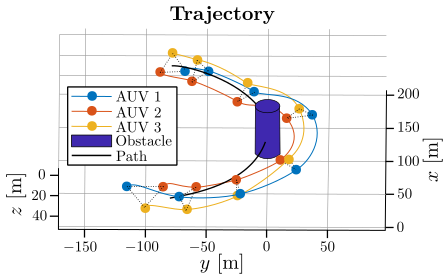
\includegraphics[width=.75\linewidth]{figures/handpos_nsb/3d_plot_alternative_view.pdf}
       \caption{The trajectory of the vehicles. The markers represent the vehicle positions every 50 seconds.}
       \label{fig:3d_plot}
   \end{subfigure}
    \begin{subfigure}[t]{.48\textwidth}
    \centering
    \def\figurewidth{.75\linewidth}
    \def\figureheight{2.5cm}
    % This file was created by matlab2tikz.
%
%The latest updates can be retrieved from
%  http://www.mathworks.com/matlabcentral/fileexchange/22022-matlab2tikz-matlab2tikz
%where you can also make suggestions and rate matlab2tikz.
%
\definecolor{mycolor1}{rgb}{0.00000,0.44700,0.74100}%
\definecolor{mycolor2}{rgb}{0.85000,0.32500,0.09800}%
\definecolor{mycolor3}{rgb}{0.92900,0.69400,0.12500}%
%
\begin{tikzpicture}

\begin{axis}[%
width=\figurewidth,
height=\figureheight,
scale only axis,
xmin=0,
xmax=350,
xlabel style={font=\color{white!15!black}},
xlabel={$t$ [s]},
ymin=-0.2,
ymax=0.25,
ylabel style={font=\color{white!15!black}, yshift=-2mm},
ylabel={Angular rate [rad/s]},
axis background/.style={fill=white},
title style={font=\bfseries, yshift=-2mm},
title={Angular velocities},
axis background/.style={fill=white},
legend style={legend cell align=left, align=left, draw=white!15!black, font=\small},
legend columns=3
]
\addplot [color=mycolor1, line width=1.0pt]
  table[]{underactuated_dynamics-1.tsv};
\addlegendentry{$p$}

\addplot [color=mycolor1, line width=1.0pt, dashed, forget plot]
  table[]{underactuated_dynamics-2.tsv};
\addplot [color=mycolor1, line width=1.0pt, dotted, forget plot]
  table[]{underactuated_dynamics-3.tsv};
\addplot [color=mycolor2, line width=1.0pt]
  table[]{underactuated_dynamics-4.tsv};
\addlegendentry{$q$}

\addplot [color=mycolor2, line width=1.0pt, dashed, forget plot]
  table[]{underactuated_dynamics-5.tsv};
\addplot [color=mycolor2, line width=1.0pt, dotted, forget plot]
  table[]{underactuated_dynamics-6.tsv};
\addplot [color=mycolor3, line width=1.0pt]
  table[]{underactuated_dynamics-7.tsv};
\addlegendentry{$r$}

\addplot [color=mycolor3, line width=1.0pt, dashed, forget plot]
  table[]{underactuated_dynamics-8.tsv};
\addplot [color=mycolor3, line width=1.0pt, dotted, forget plot]
  table[]{underactuated_dynamics-9.tsv};

\addplot[area legend, dashed, draw=black, fill=green, fill opacity=0.15, forget plot]
table[] {underactuated_dynamics-10.tsv}--cycle;
\end{axis}

\end{tikzpicture}%
    \vspace*{-6.7mm}
    \caption{The angular velocities of the vehicles. }
    \label{fig:angular_velocities}
    \end{subfigure}
    \begin{subfigure}[t]{.48\textwidth}
    \centering
    \def\figurewidth{.75\linewidth}
    \def\figureheight{2.5cm}
    % This file was created by matlab2tikz.
%
%The latest updates can be retrieved from
%  http://www.mathworks.com/matlabcentral/fileexchange/22022-matlab2tikz-matlab2tikz
%where you can also make suggestions and rate matlab2tikz.
%
\definecolor{mycolor1}{rgb}{0.00000,0.44700,0.74100}%
\definecolor{mycolor2}{rgb}{0.85000,0.32500,0.09800}%
\definecolor{mycolor3}{rgb}{0.92900,0.69400,0.12500}%
%
\begin{tikzpicture}

\begin{axis}[%
width=\figurewidth,
height=\figureheight,
scale only axis,
xmin=0,
xmax=350,
xlabel style={font=\color{white!15!black}},
xlabel={$t$ [s]},
ymin=-25,
ymax=25,
ylabel style={font=\color{white!15!black}, yshift=-2mm},
ylabel={Error [m]},
axis background/.style={fill=white},
title style={font=\bfseries, yshift=-2mm},
title={Formation keeping errors},
axis background/.style={fill=white},
legend style={legend cell align=left, align=left, draw=white!15!black,font=\scriptsize}
]
\addplot [color=mycolor1, line width=1.0pt]
table[]{formation-1.tsv};
\addlegendentry{$x$-error}

\addplot [color=mycolor1, line width=1.0pt, dashed, forget plot]
table[]{formation-2.tsv};
\addplot [color=mycolor1, line width=1.0pt, dotted, forget plot]
table[]{formation-3.tsv};
\addplot [color=mycolor2, line width=1.0pt]
table[]{formation-4.tsv};
\addlegendentry{$y$-error}

\addplot [color=mycolor2, line width=1.0pt, dashed, forget plot]
table[]{formation-5.tsv};
\addplot [color=mycolor2, line width=1.0pt, dotted, forget plot]
table[]{formation-6.tsv};
\addplot [color=mycolor3, line width=1.0pt]
table[]{formation-7.tsv};
\addlegendentry{$z$-error}

\addplot [color=mycolor3, line width=1.0pt, dashed, forget plot]
table[]{formation-8.tsv};
\addplot [color=mycolor3, line width=1.0pt, dotted, forget plot]
table[]{formation-9.tsv};

\addplot[area legend, dashed, draw=black, fill=green, fill opacity=0.15, forget plot]
table[] {formation-10.tsv}--cycle;

\addplot[area legend, dashed, draw=black, fill=white!50!red, fill opacity=0.25, forget plot]
table[] {formation-11.tsv}--cycle;
\end{axis}

\end{tikzpicture}%
    \vspace*{-6.7mm}
    \caption{The formation keeping errors. }
    \label{fig:formation_keeping_error}
    \end{subfigure}
    \begin{subfigure}[t]{.48\textwidth}
    \centering
    \def\figurewidth{.75\linewidth}
    \def\figureheight{2.5cm}
    % This file was created by matlab2tikz.
%
%The latest updates can be retrieved from
%  http://www.mathworks.com/matlabcentral/fileexchange/22022-matlab2tikz-matlab2tikz
%where you can also make suggestions and rate matlab2tikz.
%
\definecolor{mycolor1}{rgb}{0.00000,0.44700,0.74100}%
\definecolor{mycolor2}{rgb}{0.85000,0.32500,0.09800}%
%
\begin{tikzpicture}

\begin{axis}[%
width=\figurewidth,
height=\figureheight,
scale only axis,
xmin=0,
xmax=350,
xlabel style={font=\color{white!15!black}},
xlabel={$t$ [s]},
ymin=0,
ymax=25,
ylabel style={font=\color{white!15!black}, yshift=-2mm},
ylabel={Distance [m]},
axis background/.style={fill=white},
title style={font=\bfseries, yshift=-2mm},
title={Smallest distances},
legend style={at={(0.99,0.02)}, inner sep=1.5pt, anchor=south east, legend cell align=left, align=left, draw=white!15!black, legend columns=2,font=\scriptsize}
]
\addplot [color=mycolor1, line width=1.0pt]
  table[]{smallest-distances-1.tsv};
\addlegendentry{Inter-vehicle}

\addplot [color=mycolor2, line width=1.0pt]
  table[]{smallest-distances-2.tsv};
\addlegendentry{Obstacle}

\addplot [color=black, dashed, line width=1.0pt]
  table[]{smallest-distances-3.tsv};
\addlegendentry{$d_{\rm COLAV}$}


\addplot[area legend, dashed, draw=black, fill=white!50!red, fill opacity=0.25, forget plot]
table[] {smallest-distances-4.tsv}--cycle;
\end{axis}

\end{tikzpicture}%

    \vspace*{-1.8mm}
    \caption{The minimum inter-vehicle and vehicle to obstacle distance.}
    \label{fig:collision_avoidance}
    \end{subfigure}
    \begin{subfigure}[t]{.48\textwidth}
    \centering
    \def\figurewidth{.75\linewidth}
    \def\figureheight{2.5cm}
    % This file was created by matlab2tikz.
%
%The latest updates can be retrieved from
%  http://www.mathworks.com/matlabcentral/fileexchange/22022-matlab2tikz-matlab2tikz
%where you can also make suggestions and rate matlab2tikz.
%
\definecolor{mycolor1}{rgb}{0.00000,0.44700,0.74100}%
\definecolor{mycolor2}{rgb}{0.85000,0.32500,0.09800}%
\definecolor{mycolor3}{rgb}{0.92900,0.69400,0.12500}%
%
\begin{tikzpicture}

\begin{axis}[%
width=\figurewidth,
height=\figureheight,
scale only axis,
xmin=0,
xmax=350,
xlabel style={font=\color{white!15!black}},
xlabel={$t$ [s]},
ymin=-20,
ymax=20,
ylabel style={font=\color{white!15!black}, yshift=-1.5mm},
ylabel={Error [m]},
axis background/.style={fill=white},
title style={font=\bfseries, yshift=-2.75mm},
title={Path following error},
legend style={legend cell align=left, align=left, draw=white!15!black,font=\scriptsize, at={(0.99, 0.01)}, anchor=south east}
]
\addplot [color=mycolor1, line width=1.0pt]
  table[]{path-following-1.tsv};
\addlegendentry{$x$-error}

\addplot [color=mycolor2, line width=1.0pt]
  table[]{path-following-2.tsv};
\addlegendentry{$y$-error}

\addplot [color=mycolor3, line width=1.0pt]
  table[]{path-following-3.tsv};
\addlegendentry{$z$-error}


\addplot[area legend, dashed, draw=black, fill=green, fill opacity=0.15, forget plot]
table[] {path-following-4.tsv}--cycle;
\end{axis}

\end{tikzpicture}%

    \vspace*{-6.7mm}
    \caption{The barycenter path-following error.}
    \label{fig:path_following_error}
    \end{subfigure}
    \caption{Simulation results of the path-following algorithm proposed in Section~\ref{sec:case_study}. The full, dashed, and dotted lines correspond to the three different vehicles. The green and red rectangles represent when obstacle avoidance and inter-vehicle COLAV is active.}
    \label{fig:sim_results}
\end{figure}

The resulting trajectory of the mission is shown in \figref{fig:3d_plot}. The vehicles avoid the obstacle with a margin and return to the desired path. \figref{fig:angular_velocities} shows that the angular velocities remain bounded, in accordance with Proposition~\ref{prop:angular_velocities}. \figref{fig:formation_keeping_error} shows that the fleet converges to the desired formation while the obstacle avoidance mode is active. Except for during the inter-vehicle collision avoidance, the convergence seems linear, which can be expected because the task velocity is saturated by $v_{2,\max}$. \figref{fig:collision_avoidance} shows that the inter-vehicle \gls{colav} task activates when the distance between vehicles is below $d_{COLAV}$, and the distance does not decrease further. Because the obstacle avoidance radius $r_o$ was chosen $10 \mathrm{m}$ wider than the obstacle, the obstacle is avoided with a $10 \mathrm{m}$ margin. \figref{fig:path_following_error} shows that the path-following error initially increases as the fleet avoids the obstacle because the $x$- and $y$-components of $\mathbf{v}_{LOS,d}$ and $\dot{\mathbf{v}}_{LOS,d}$ are replaced with $\mathbf{v}_{OA,d}$ and $\dot{\mathbf{v}}_{OA,d}$ given by \eqref{eq:v_OA}, \eqref{eq:v_OA_dot}. As expected from Theorem~\ref{theorem:path_error}, the error converges to zero after the obstacle is passed when the LOS task is activated again.

\section{Conclusions and Future Work}\label{sec:conclusion}
%%%%%%%%%%%%%%%%%%%%%%%%%%%%%%%%%%%%%%%%%%%%%%%%%%%%%%%%%%%%%%%%%%%%%%%%%%%%%%%%

In this chapter, we proposed an extended \gls{nsb} method for double-integrator systems. The method was proved to provide \acrlongpl{ges} task error dynamics. The method was demonstrated in a case study of formation path-following with underactuated \glspl{auv}. We defined the second-order kinematic tasks for collision avoidance, formation-keeping, and path-following. To force a bounded velocity, we introduced a saturation term to the formation-keeping acceleration. The closed-loop formation-error system with the reformulated formation-keeping acceleration was proved to be \glspl{ugas}, and the closed-loop path-following system was proved to be \glspl{usges}. Simulation results demonstrate the effectiveness of our approach. Possible future work includes verifying the presented results through experiments.
